\documentclass[handout]{beamer}
\usepackage[T1]{fontenc}
\usepackage[utf8]{inputenc}
\usepackage{lmodern}
\usepackage[italian]{babel}

\title{Creazione di un curriculum}
\author{Mattia Cozzi}
\date{a.f.~2024/2025}


%\documentclass[handout]{beamer}     %usare questa classe per generare l'handout

%\usepackage{pdfpages}   %per mostrare più quadri nella stessa pagina
%\pgfpagesuselayout{4 on 1}[a4paper,border shrink=5mm,landscape]


\usetheme{Singapore}
%\useoutertheme[left]{sidebar} %elementi intorno alle diapositive
\setbeamercovered{dynamic} %modifica l'aspetto del testo grigetto delle diapositive future. Argomenti: invisible/transparent/dynamic


%COLORE PRINCIPALE
\definecolor{verde}{RGB}{2, 194, 117} % UBC Blue (primary)
\setbeamercolor{structure}{fg=verde} % itemize, enumerate, etc
\setbeamercolor{alerted text}{fg=verde}


\usecolortheme{orchid}

\usepackage{tikz}

\begin{document}

\begin{frame}
  \titlepage
\end{frame}


\begin{frame}
\frametitle{Contenuti}
\tableofcontents
\end{frame}



\section{Introduzione}


\begin{frame}
\frametitle{Ricerca di personale}
Quando un'azienda è alla ricerca di personale \alert{può muoversi in maniera diversa} a seconda della figura ricercata, della propria cultura aziendale ed della propria policy di selezione e gestione del personale.\pause

~

Le aziende medio-grandi hanno un reparto che si occupa di selezione e gestione del personale (\alert{HR}, \emph{human resources}).\pause

~

Nelle aziende più piccole (ad esempio a conduzione familiare) può essere direttamente il/la titolare o un suo incaricato/a a gestire la fase di selezione.
\end{frame}

\begin{frame}
\frametitle{Modalità di ricerca di personale (1)}
Esistono diversi modi di trovare nuovi lavoratori e lavoratrici:
\begin{itemize}
  \item \alert{informalmente}, attivando la propria rete di relazioni, chiedendo di segnare nominativi di persone valide;{\pause} in questi casi può prevalere il rapporto di fiducia con chi consiglia il personale, a scapito della valutazione delle competenze.
\end{itemize}
\visible<2->{\begin{figure}
  
\includegraphics[width=.6\columnwidth]{img/conversazione.jpg}
\end{figure}}
\end{frame}

\begin{frame}
\frametitle{Modalità di ricerca di personale (2)}
\begin{itemize}\setcounter{enumi}{1}
  \item con \alert{banche dati interne e sito aziendale}, cioè cercando tra i curricula che ricevono (\alert{candidatura spontanea}) o attivando la sezione ``Carriere/Lavora con noi'' del loro sito web.
\end{itemize}
\begin{figure}
  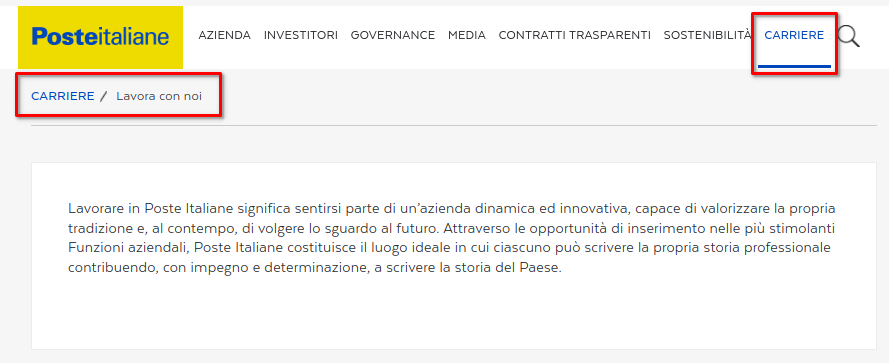
\includegraphics[width=.8\columnwidth]{img/lavoraconnoi.png}
\end{figure}
\end{frame}


\begin{frame}
\frametitle{Modalità di ricerca di personale (3)}
\begin{itemize}\setcounter{enumi}{1}
  \item con \alert{annunci su giornali e portali online}, come \href{https://www.linkedin.com/}{LinkedIn}, \href{https://it.indeed.com/}{Indeed} o \href{https://www.infojobs.it/}{Infojobs}; in questi casi bisogna essere molto attenti ad evitare truffe e raggiri, diffidare di chi offre guadagni rapidi e da annunci senza informazioni.
\end{itemize}
\begin{figure}
  
\includegraphics[width=.8\columnwidth]{img/indeed.png}
\end{figure}
\end{frame}



\begin{frame}
\frametitle{Modalità di ricerca di personale (4)}
\begin{itemize}\setcounter{enumi}{1}
  \item con \alert{intermediari}, come centri per l'impiego, centri di formazione professionale o agenzie di ricerca e selezione personale;{\pause} queste ultime sono dette anche \alert{agenzie interinali}, come Adecco, Randstad, Etjca, ecc.
\end{itemize}
\visible<2->{\begin{figure}
  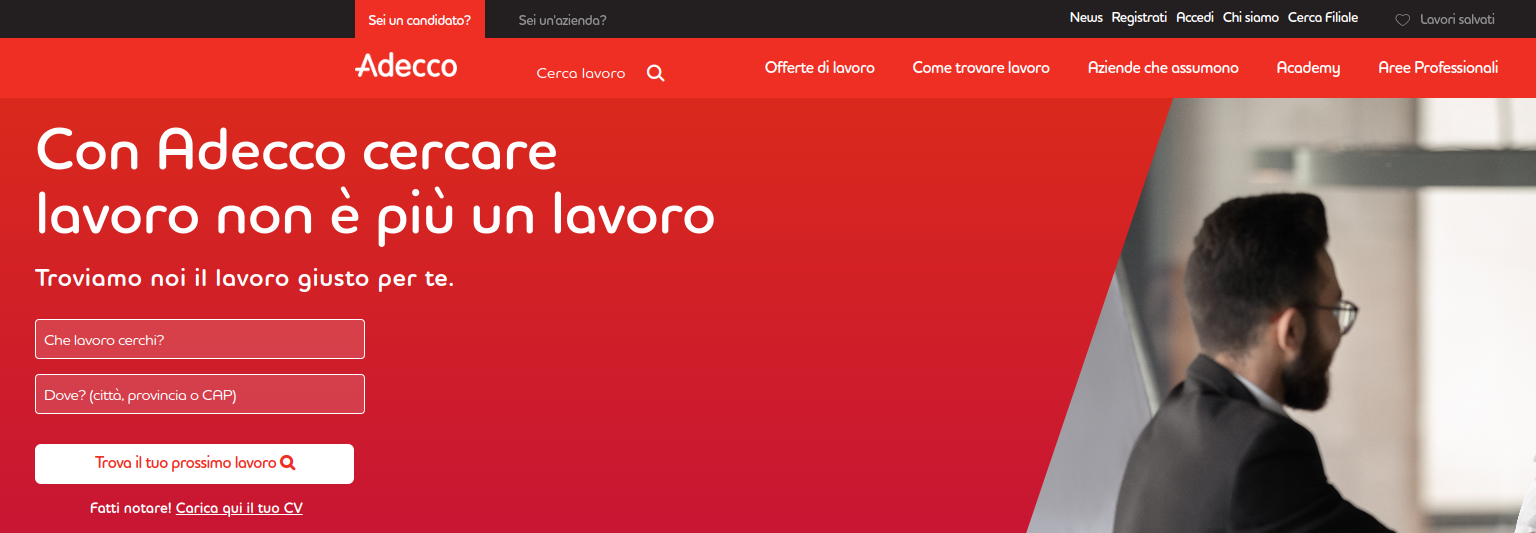
\includegraphics[width=.8\columnwidth]{img/adecco.png}
\end{figure}}
\end{frame}



\begin{frame}
\frametitle{Cos'è il curriculum}
Il termine \alert{curriculum vitae} viene dal latino e significa ``percorso di vita'': serve a presentare la propria situazione personale, scolastica e lavorativa.\pause

~

È una sorta di ``biglietto da visita professionale'', con cui proporsi per un posto e partecipare alla selezione di personale.\pause

~

È la prima cosa che viene richiesta durante la ricerca di un lavoro, ed è ciò che usiamo per \alert{arrivare ad un colloquio di lavoro}.
\end{frame}


\begin{frame}
\frametitle{Curriculum efficace e non efficace}
È importante preparare CV \alert{mirati e personalizzati} in base all'azienda che stiamo contattando e per il profilo per il quale ci stiamo candidando.\pause

~

Con un buon CV dobbiamo:
\begin{itemize}
  \item comunicare informazioni \alert{interessanti};\pause
  \item comunicare informazioni \alert{pertinenti};\pause
  \item \alert{incuriosire} il lettore.
\end{itemize}
\end{frame}


\begin{frame}
\frametitle{Caratteristiche fondamentali di un buon CV}
Un buon curriculum deve essere:
\begin{itemize}
  \item \alert{completo}, con tutte le informazioni utili su di noi, sia lavorativamente sia sulla nostra personalità;\pause
  \item \alert{sintetico}, evitando frasi ridondanti, lungo al massimo due pagine;\pause
  \item \alert{chiaro e comunicativo}, scritto al computer e facendo risaltare le informazioni più interessanti;\pause
  \item \alert{mirato}, scritto in modo da avvicinarsi il più possibile, senza mentire, alla posizione per cui ci candidiamo.
\end{itemize}
\end{frame}

\section{Contenuto}


\begin{frame}
\frametitle{Dati da indicare necessariamente}
\begin{itemize}
  \item Nome e cognome;\pause
  \item residenza;\pause
  \item numero di telefono e indirizzo email;\pause
  \item possesso patente/i e mezzi di trasporto;\pause
  \item percorso di istruzione e formazione (quanto basta);\pause
  \item esperienze professionali precedenti, con riferimenti specifici a luoghi e date;\pause
  \item stage e tirocini;\pause
  \item conoscenze tecniche (\emph{hard skills});\pause
  \item conoscenze linguistiche (con livello di padronanza);\pause
  \item conoscenze informatiche (con livello di padronanza);\pause
  \item competenze trasversali (\emph{soft skills}: capacità di organizzare il lavoro, rapporto coi colleghi, ecc.).
\end{itemize}
\end{frame}

\begin{frame}
\frametitle{Devo scrivere tutto?}
Dati da riportare se richiesto:
\begin{itemize}
  \item data di nascita;\pause
  \item fotografia (primo piano, sfondo neutro).\pause
\end{itemize}

~

Dati da non riportare:
\begin{itemize}
  \item segno zodiacale;\pause
  \item informazioni inutili su di noi;\pause
  \item dati fisici, a meno che non siano richiesti per lavoro (es.~modella).\pause
\end{itemize}

~

Non ci devono essere errori grammaticali o di battitura!\pause

~

Attenzione a riportare i propri contatti social, può essere un'arma a doppio taglio!
\end{frame}


\begin{frame}
\frametitle{Esperienze non lavorative}
Inserire le esperienze non lavorative nel curriculum a volte può \alert{fare la differenza}.\pause

~

Aver partecipato ad incontri, corsi di formazione, attività di volontariato ed altre esperienze attinenti al ruolo che si andrà a ricoprire potrebbe essere decisivo per un'assunzione.\pause

~

Di fronte ad un altro profilo con un percorso professionale e formativo pari o simile al nostro, il selezionatore potrebbe decidere di darci un'occasione proprio in virtù della nostra \alert{esperienza al di fuori del lavoro}.
\end{frame}



\begin{frame}
\frametitle{Soft skills}
Alcuni esempi di \emph{soft skills}:
\begin{itemize}
  \item essere creativi/e;\pause
  \item essere in grado di prendere decisioni;\pause
  \item possedere l'intelligenza emotiva, cioè saper ascoltare e capire come stanno le persone intorno a noi;\pause
  \item saper fare Problem Solving, cioè ragionare per risolvere problemi;\pause
  \item capacità di gestire un gruppo;\pause
  \item saper gestire lo stress;\pause
  \item essere proattivo/a, cioè saper prendere iniziative senza subire le decisioni degli altri.
\end{itemize}
  

\end{frame}


\begin{frame}
\frametitle{Consenso al trattamento dei dati}
Uno degli errori più comuni frequenti nella scrittura di un CV è quello di \alert{dimenticarsi di inserire l'autorizzazione al trattamento dei dati personali}.\pause

~

Inserirla significa autorizzare chi riceve il CV ad analizzare ed usare i dati del candidato/a, che sono tutelati dalla legge sulla privacy.\pause

~

In sostanza, senza quella dicitura legalmente le aziende non potrebbero contattarti. È quindi importante ricordarsi di inserirla in basso nell’ultima pagina del CV, con data e firma.
\end{frame}


\begin{frame}
\frametitle{Dicitura standard per il trattamendo dei dati}
Esistono diverse formule per acconsentire al trattamento dei dati personali, come ad esempio:

~

\begin{quote}
  Autorizzo il trattamento dei dati personali contenuti nel mio curriculum vitae in base al \alert{Dlgs 196 del 30 giugno 2003} e all’\alert{art. 13 del GDPR}.
\end{quote}\pause

~

~

Ricorda infine sempre di \alert{datare e firmare il CV}!
\end{frame}



\section{Europass}

\begin{frame}
\frametitle{Europass}
\begin{figure}
  
\includegraphics[width=.35\columnwidth]{img/europass.png}
\end{figure}
Il Curriculum Vitae europeo, o Europass, è un formato introdotto a partire dal 2002 dalla Commissione Europea. È un \alert{modello standard} e permette una lettura rapida e chiara del CV per poterlo confrontare velocemente con altri.\pause

~

Il CV europeo ha una struttura semplice e lineare ed è diviso in sezioni con un \alert{layout a colonne}.
\end{frame}


\begin{frame}
\frametitle{Esempio di CV in formato europeo}
\begin{figure}
  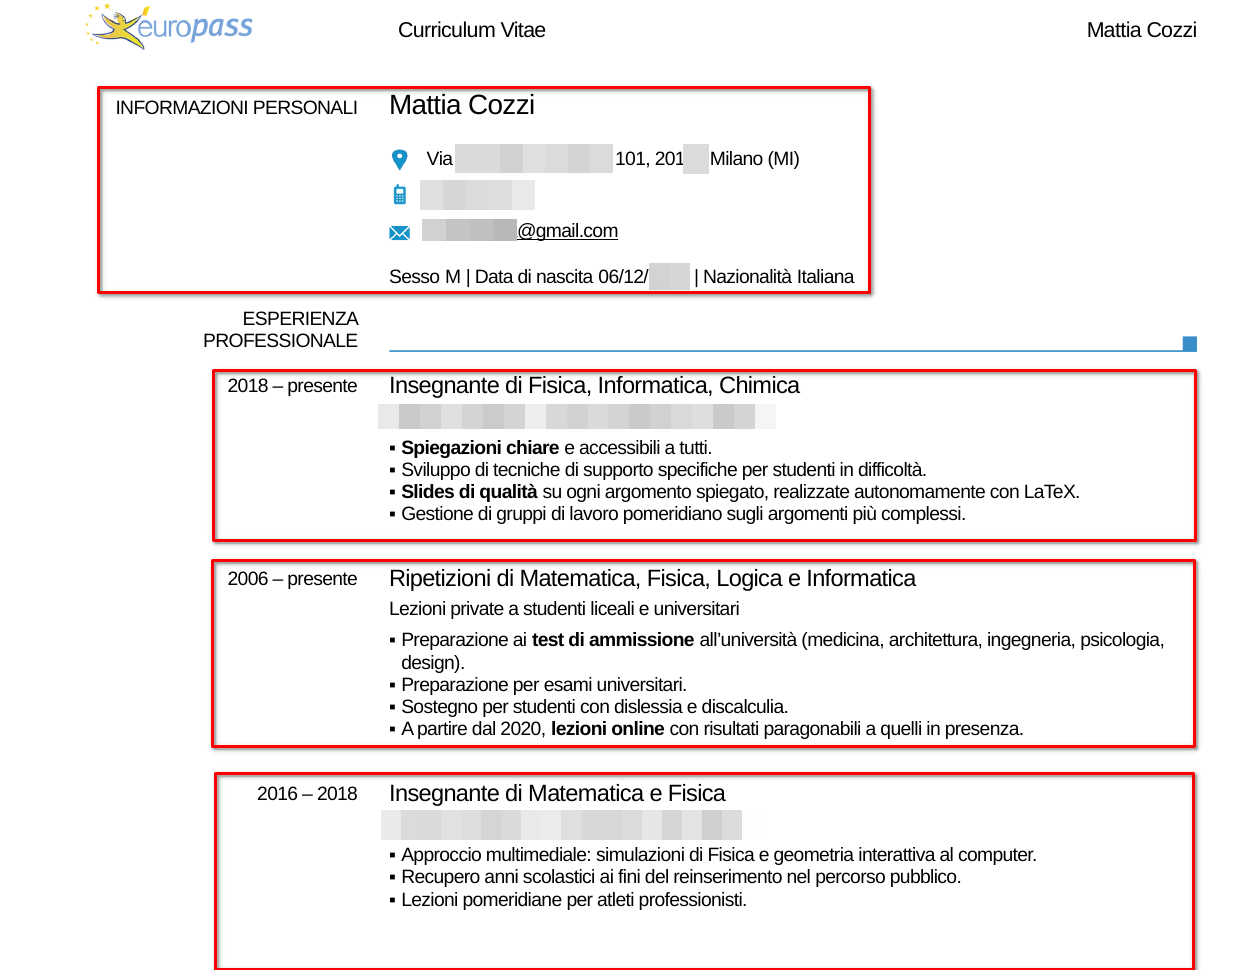
\includegraphics[width=.9\columnwidth]{img/cveuromc.png}
\end{figure}
\end{frame}

\begin{frame}
\frametitle{Vantaggi e svantaggi}
Il Curriculum Vitae europeo è il formato ideale per chi sta valutando l'idea di cercare lavoro all'estero e per chi non ha molte esperienze di lavoro da illustrare.\pause

~

Se invece hai molte esperienze lavorative alle spalle o un importante percorso di formazione, l'Europass potrebbe non essere il modello più indicato da utilizzare, poiché mette a disposizione poco spazio.\pause

~

Ha inoltre lo svantaggio di non essere particolarmente ``interessante'', quindi se stiamo cercando lavori più creativi può essere utile anche creare un CV di un altro tipo.
\end{frame}



\begin{frame}
\frametitle{CV europeo online}
Dal sito \href{https://europass.europa.eu/it}{https://europass.europa.eu/it} è possibile seguire una \alert{procedura guidata} per la creazione del proprio curriculum europeo.

~

\begin{figure}
  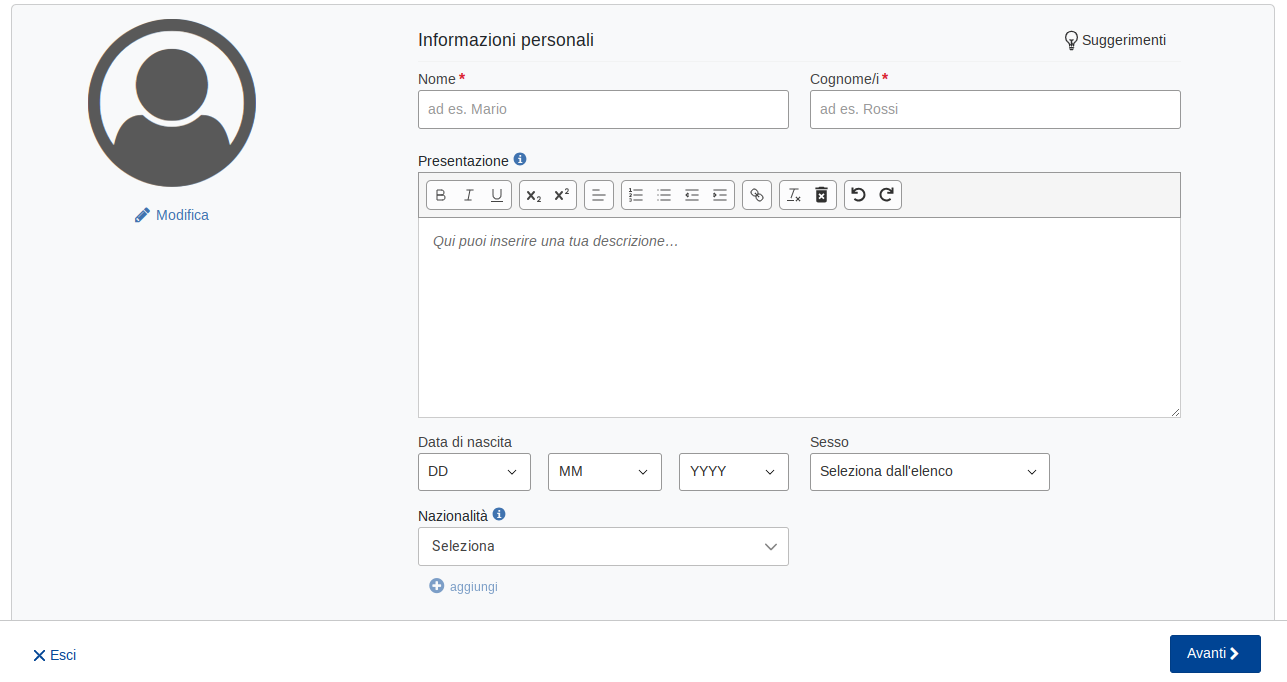
\includegraphics[width=.8\columnwidth]{img/cvonline.png}
\end{figure}
\end{frame}

\begin{frame}
\frametitle{Modelli online}
Per crearlo sul nostro computer esistono dei \alert{template preimpostati} e modificabili che si trovano facilmente su Internet.\pause

~

Con una rapida ricerca su Google di ``modello cv europass'' troviamo:
\begin{center}
  \href{https://www.governo.it/sites/governo.it/files/cvformatoeuropeoB.doc}{www.governo.it/sites/governo.it/files/cvformatoeuropeoB.doc}
\end{center}
che scarichiamo e possiamo modificare con Word.
\end{frame}

\begin{frame}
\frametitle{Template Europass modificabile}
\begin{figure}
  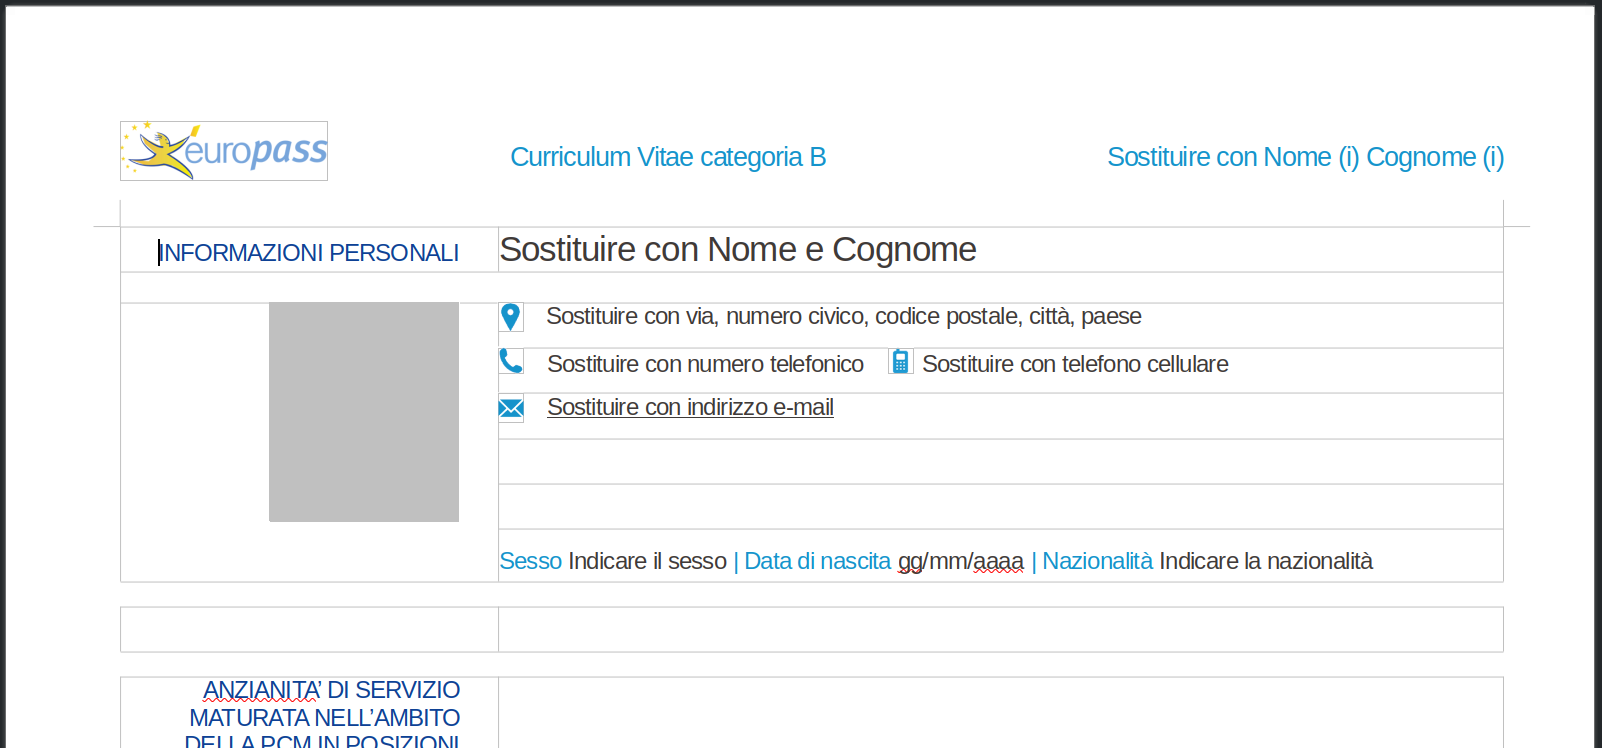
\includegraphics[width=\columnwidth]{img/cvtemplate.png}
\end{figure}

Il file scaricato è organizzato con delle \alert{caselle di testo}, che andremo a riempire coi nostri dati.
\end{frame}


\begin{frame}
\frametitle{Esercizi}
\begin{enumerate}
  \item Crea il tuo \alert{curriculum reale}, modificando il modello proposto in queste slides. Aggiungi anche la tua foto e i tuoi contatti. Salvalo in formato PDF, stampalo e firmalo.
  
  ~
  \item Crea il curriculum di un \alert{personaggio immaginario} che si sta candidando per la posizione di manager di un supermercato molto grande in provincia di Milano. Salvalo in formato PDF.
\end{enumerate}
\end{frame}


\section{Altri modelli}

\begin{frame}
\frametitle{Altri tipi di CV}
Il tuo Cv potrebbe assumere anche le sembianze diverse dal tradizionale formato Europass: se non vuoi crearne uno, puoi ricorrere ai moltissimi modelli presenti online.\pause

~

I formati alternativi hanno il vantaggio di poter realizzare CV creativi, chiari, diretti mettendo a disposizione di chi legge (\alert{in un unico foglio}) le informazioni che vuoi comunicare e mettere in evidenza.\pause

~

Un ottimo strumento per realizzare un CV non Europass è \alert{Canva}. Canva è gratuito nelle sue funzioni base (che sono molte), a pagamento per quelle avanzate.
\end{frame}

\begin{frame}
\frametitle{Esempi di CV non Europass}
\begin{columns}
  \begin{column}{.45\textwidth}
    \begin{figure}
      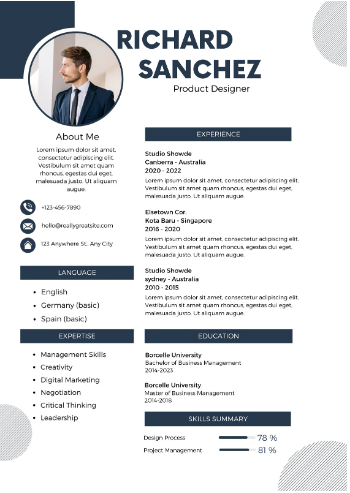
\includegraphics[width=\columnwidth]{img/cv1.png}
    \end{figure} 
  \end{column}
  \begin{column}{.45\textwidth}
    \begin{figure}
      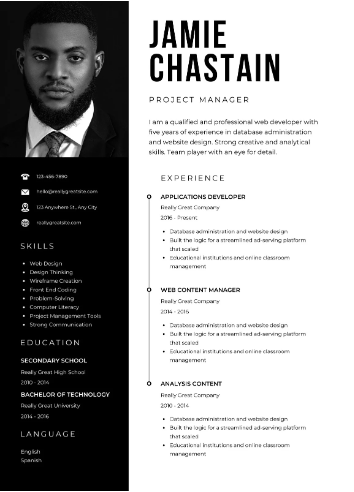
\includegraphics[width=\columnwidth]{img/cv2.png}
    \end{figure}
  \end{column}
\end{columns}
\end{frame}

\begin{frame}
\frametitle{Esempi di CV non Europass}
\begin{columns}
  \begin{column}{.45\textwidth}
    \begin{figure}
      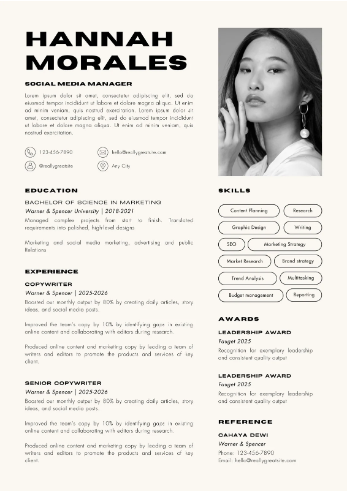
\includegraphics[width=\columnwidth]{img/cv3.png}
    \end{figure} 
  \end{column}
  \begin{column}{.45\textwidth}
    \begin{figure}
      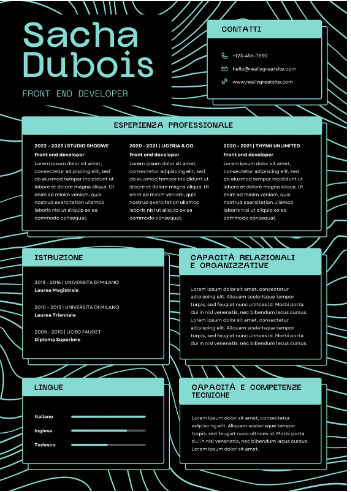
\includegraphics[width=\columnwidth]{img/cv4.png}
    \end{figure}
  \end{column}
\end{columns}
\end{frame}



\begin{frame}
\frametitle{Infografica}
Un esempio di CV alternativo è la creazione di un'\alert{infografica} che contiene le informazioni su di te, un modo originale e immediato di presentarti.\pause

\begin{columns}
  \begin{column}{.4\textwidth}
    I tuoi dati anagrafici, la tua formazione, le tue esperienze e competenze saranno tradotti in un formato grafico: si tratta infatti di una
    trasposizione grafica e visiva di informazioni.
  \end{column}
  \begin{column}{.4\textwidth}
    \begin{figure}
      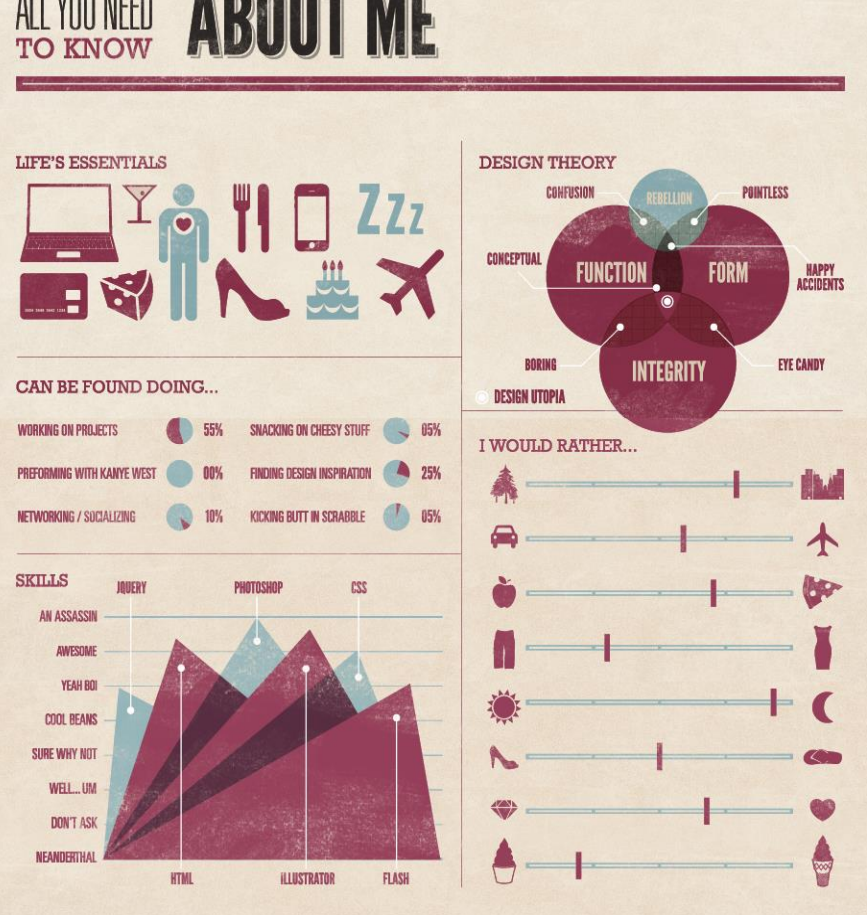
\includegraphics[width=\columnwidth]{img/cvinfografica.png}
    \end{figure}
  \end{column}
\end{columns}
\end{frame}



\begin{frame}
\frametitle{Esempi di CV infografica}
\begin{columns}
  \begin{column}{.45\textwidth}
    \begin{figure}
      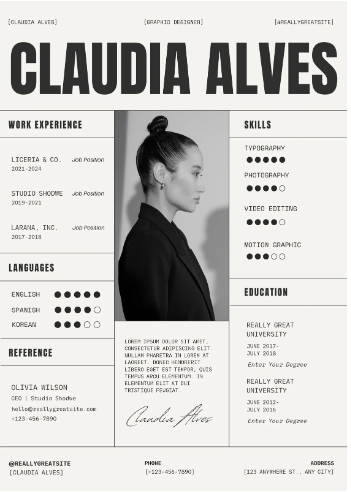
\includegraphics[width=\columnwidth]{img/cv5.png}
    \end{figure} 
  \end{column}
  \begin{column}{.45\textwidth}
    \begin{figure}
      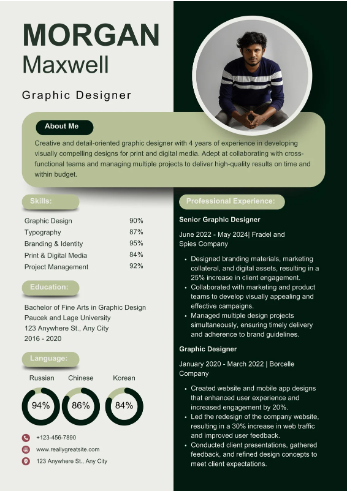
\includegraphics[width=\columnwidth]{img/cv6.png}
    \end{figure}
  \end{column}
\end{columns}
\end{frame}


\begin{frame}
\frametitle{Esempi di CV infografica}
\begin{columns}
  \begin{column}{.45\textwidth}
    \begin{figure}
      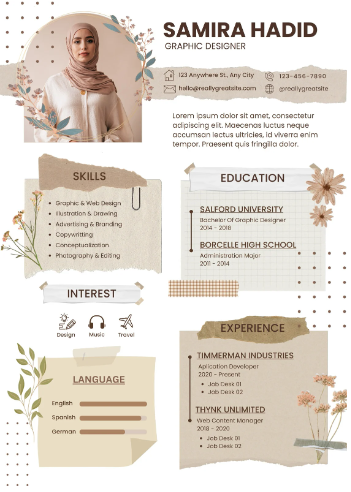
\includegraphics[width=\columnwidth]{img/cv7.png}
    \end{figure} 
  \end{column}
  \begin{column}{.45\textwidth}
    \begin{figure}
      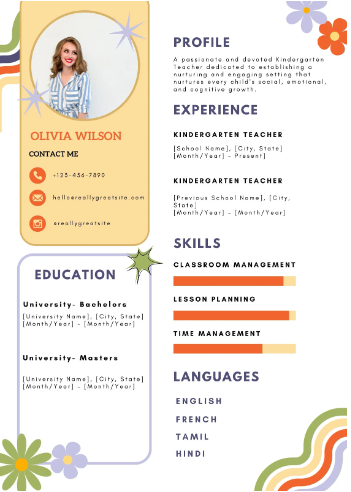
\includegraphics[width=\columnwidth]{img/cv8.png}
    \end{figure}
  \end{column}
\end{columns}
\end{frame}



\section{Presentazione}

\begin{frame}
\frametitle{La lettera di presentazione}
La lettera di presentazione è solitamente una mail che ha lo scopo di indicare la ragione per cui si è inviato il curriculum vitae e deve evidenziare brevemente i punti forti di chi scrive.\pause

~

La lettera di presentazione è la naturale ``compagna del curriculum'' e deve invogliare il selezionatore a leggere il curriculum allegato.

\begin{figure}
  
\includegraphics[width=\columnwidth]{img/lettera.jpg}
\end{figure}
\end{frame}

\begin{frame}
\frametitle{Impostazione della lettera}
A seconda che si risponda ad un annuncio o ci si autocandidi, la lettera deve essere impostata in modo diverso:

~
\begin{itemize}
  \item quando ci si \alert{autocandida}, la lettera d'accompagnamento deve far comprendere al selezionatore il tipo di lavoro che si vorrebbe ricoprire all’interno di quella azienda e soprattutto i motivi per cui si potrebbe essere un utile collaboratore;\pause
  
  ~

  \item nel caso di risposta ad un \alert{annuncio}, la lettera deve indicare perché si è interessati a quella mansione e le caratteristiche personali utili a ricoprire il ruolo richiesto nell’annuncio.
\end{itemize}
\end{frame}
 

\begin{frame}
\frametitle{Elementi della lettera di presentazione}
La lettera deve indicare:
\begin{itemize}
  \item intestazione con i nostri dati principali;
  \item luogo e data;
  \item destinatario (ad esempio il/la titolare, il direttore del personale o l'ufficio selezione del personale);
  \item oggetto;
  \item testo principale;
  \item firma.
\end{itemize}
\end{frame}

\begin{frame}
\frametitle{Esempio di lettera di presentazione (1)}
\small
``Gentile [referente],

con la presente esprimo il mio interesse per la posizione di [ruolo] presso [azienda].

Il mio interesse per [settore] mi ha portato da (esperienza) a (esperienza). Credo fermamente che la mia passione per [background o settore] / l’interesse per [aspetto del campo di lavoro] / il grande impegno per [settore], mi rendano il candidato ideale per entrare a far parte del vostro team.

Potrei, infatti, mettere immediatamente in campo la mia esperienza in materia di [elencare le skills]:
\begin{itemize}
  \item (skill 1)
  \item \ldots
\end{itemize}
\end{frame}



\begin{frame}
\frametitle{Esempio di lettera di presentazione (2)}
\small
Nel mio precedente ruolo di [lavoro precedente] ho infatti [spiegare brevemente il progetto, le proprie mansioni, gli obiettivi raggiunti]. Questa esperienza mi ha permesso di mettere in campo/acquisire capacità di [skills].

Attualmente sono alla ricerca di una nuova opportunità professionale che mi permetta di mettere a frutto le mie competenze in materia, e ritengo che [nome azienda] sia il luogo ideale per farlo, così come io posso essere una risorsa in grado di apportare valore aggiunto.

Spero di avere l’opportunità di incontrarla di persona.

Grazie per l’attenzione.

Cordiali saluti,

[Nome e cognome]

[recapiti email e telefono].''
\end{frame}

\begin{frame}
\frametitle{Esercizio}
\begin{enumerate}
  \item Immagina di rispondere ad un annuncio per il lavoro che preferisci e crea la tua \alert{lettera di presentazione}. Salvala in formato PDF, stampala e firmala.
\end{enumerate}
\end{frame}

\section{Portfolio}

\begin{frame}
\frametitle{Cos'è un portfolio?}
Per i lavori più creativi, può essere utile e interessante creare un portfolio.\pause

~

Un portfolio è una \alert{raccolta strutturata} dei propri lavori, disegni, fotografie o altro.\pause

~

Un portfolio può assumere la forma di una o più pagine, di un video o di un intero sito web dedicato.
\end{frame}

\begin{frame}
\frametitle{Esempi di portfolio}
\begin{center}
  Portfolio cartaceo: 
  
  \href{http://www.gerardopulido.com/uploads/contenidos/portfolio_gpulido.pdf}{http://www.gerardopulido.com/\ldots/portfolio\_gpulido.pdf}

  ~

  ~

  Video portfolio:
  
  \href{https://www.youtube.com/watch?v=Vgj9meWvsjQ}{https://www.youtube.com/watch?v=Vgj9meWvsjQ}

  ~

  ~

  Sito web:
  
  \href{https://548487.my.canva.site/}{https://548487.my.canva.site/}
\end{center}
\end{frame}


\begin{frame}
\frametitle{Canva per il portfolio}
Canva propone anche molti modelli (anche animati) di portfolio.\pause

~

\begin{figure}
  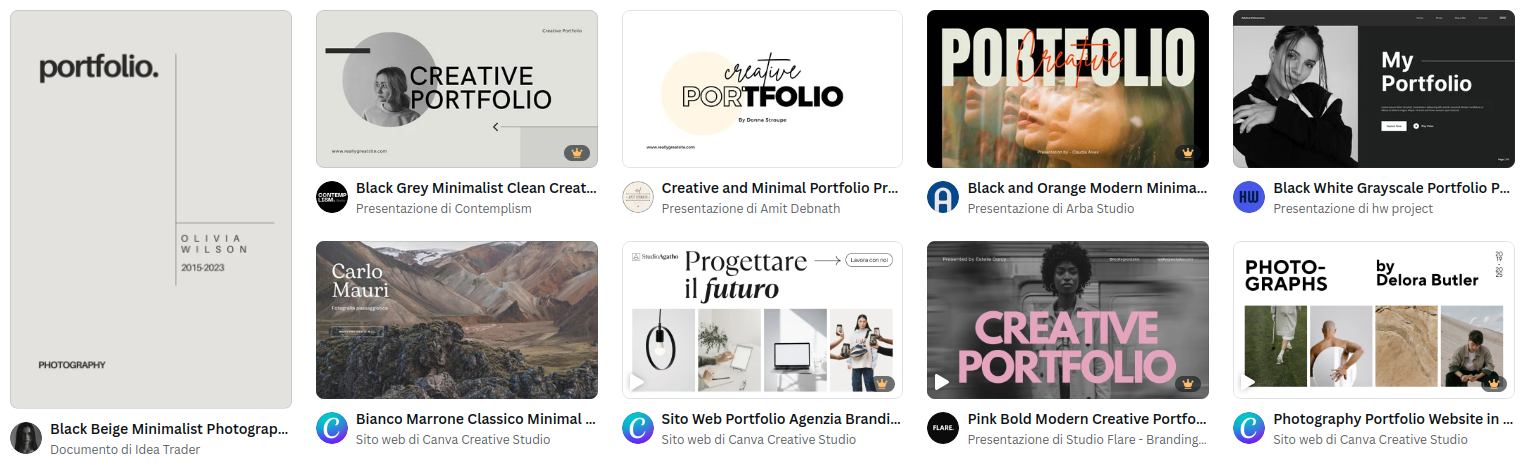
\includegraphics[width=\columnwidth]{img/portfoliocanva.png}
\end{figure}

~

Una volta inseriti gli elementi che desideriamo, possiamo salvarlo come PDF oppure creare un intero sito web con un URL personalizzato.
\end{frame}

\end{document}
